\documentclass{standalone}
\usepackage{tikz}
\usetikzlibrary{patterns, positioning}


\begin{document}
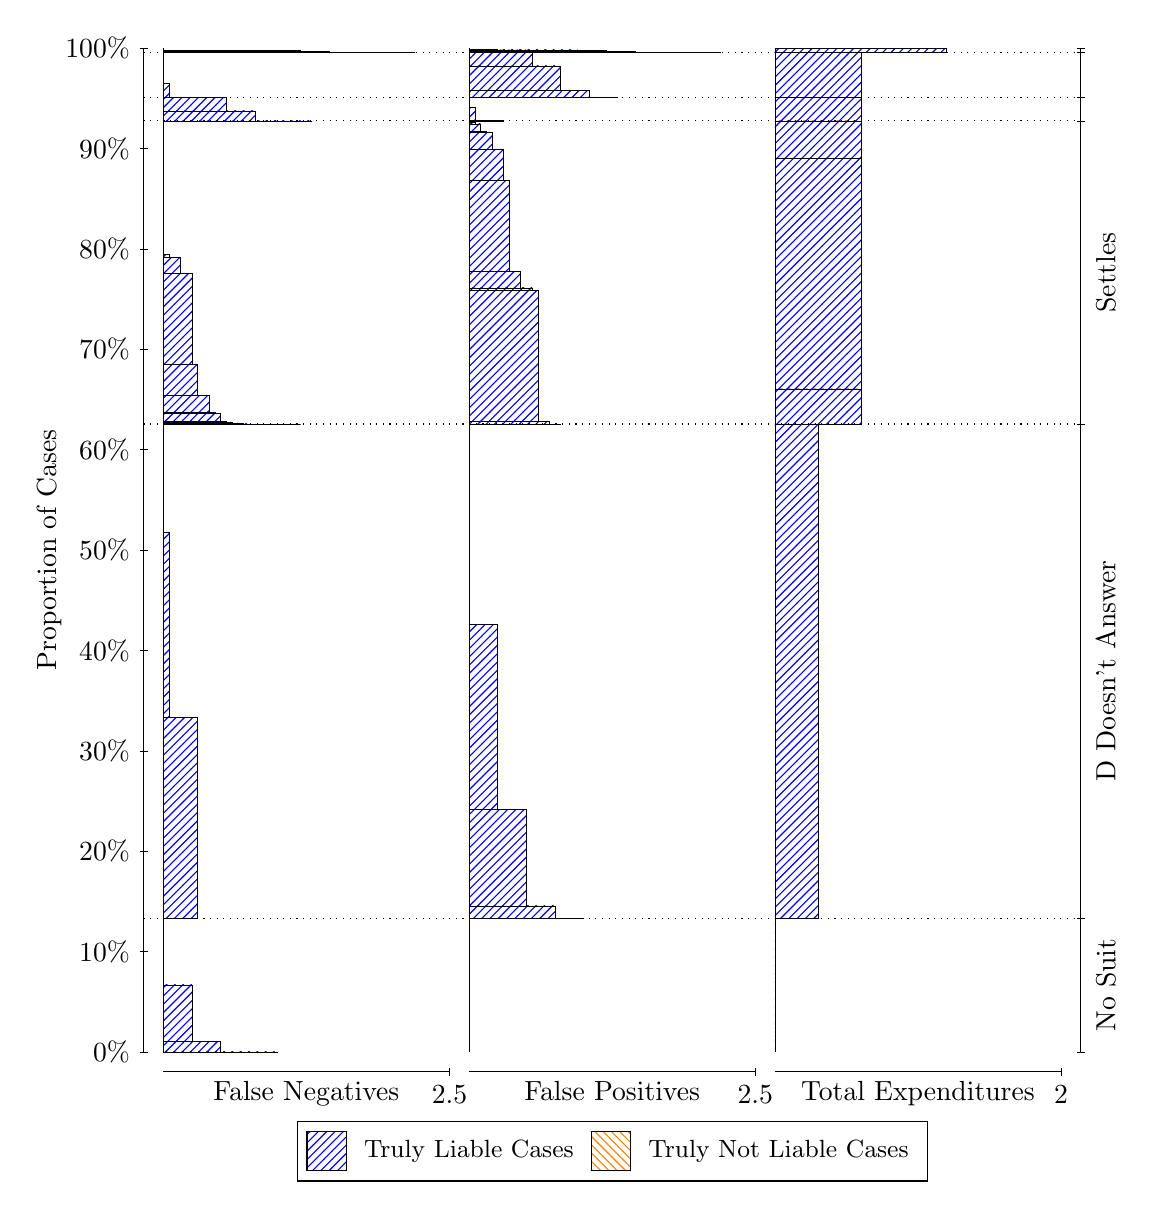
\begin{tikzpicture}
\draw[black, very thin] (1.5,1.75) -- (1.5,14.5);
\node[rotate=90, text=black, anchor=center] at (0.3, 8.125) {Proportion of Cases};
\draw[black, very thin] (1.45,1.75) -- (1.55,1.75);
\node[text=black, anchor=east] at (1.45, 1.75) {0\%};
\draw[black, very thin] (1.45,3.025) -- (1.55,3.025);
\node[text=black, anchor=east] at (1.45, 3.025) {10\%};
\draw[black, very thin] (1.45,4.3) -- (1.55,4.3);
\node[text=black, anchor=east] at (1.45, 4.3) {20\%};
\draw[black, very thin] (1.45,5.575) -- (1.55,5.575);
\node[text=black, anchor=east] at (1.45, 5.575) {30\%};
\draw[black, very thin] (1.45,6.85) -- (1.55,6.85);
\node[text=black, anchor=east] at (1.45, 6.85) {40\%};
\draw[black, very thin] (1.45,8.125) -- (1.55,8.125);
\node[text=black, anchor=east] at (1.45, 8.125) {50\%};
\draw[black, very thin] (1.45,9.4) -- (1.55,9.4);
\node[text=black, anchor=east] at (1.45, 9.4) {60\%};
\draw[black, very thin] (1.45,10.675) -- (1.55,10.675);
\node[text=black, anchor=east] at (1.45, 10.675) {70\%};
\draw[black, very thin] (1.45,11.95) -- (1.55,11.95);
\node[text=black, anchor=east] at (1.45, 11.95) {80\%};
\draw[black, very thin] (1.45,13.225) -- (1.55,13.225);
\node[text=black, anchor=east] at (1.45, 13.225) {90\%};
\draw[black, very thin] (1.45,14.5) -- (1.55,14.5);
\node[text=black, anchor=east] at (1.45, 14.5) {100\%};

\draw[black, very thin] (13.4,1.75) -- (13.4,14.5);
\draw[black, very thin] (13.35,1.75) -- (13.45,1.75);
\node[anchor=west] at (13.35, 1.75) {};
\draw[black, very thin] (13.35,3.4496) -- (13.45,3.4496);
\node[anchor=west] at (13.35, 3.4496) {};
\draw[black, very thin] (13.35,9.725) -- (13.45,9.725);
\node[anchor=west] at (13.35, 9.725) {};
\draw[black, very thin] (13.35,13.574) -- (13.45,13.574);
\node[anchor=west] at (13.35, 13.574) {};
\draw[black, very thin] (13.35,13.873) -- (13.45,13.873);
\node[anchor=west] at (13.35, 13.873) {};
\draw[black, very thin] (13.35,14.446) -- (13.45,14.446);
\node[anchor=west] at (13.35, 14.446) {};
\draw[black, very thin] (13.35,14.5) -- (13.45,14.5);
\node[anchor=west] at (13.35, 14.5) {};

\draw[black, very thin, pattern color=blue, pattern=north east lines] (1.75,1.75) rectangle (3.2033,1.75);
\draw[black, very thin, pattern color=blue, pattern=north east lines] (1.75,1.75) rectangle (2.84,1.7511);
\draw[black, very thin, pattern color=blue, pattern=north east lines] (1.75,1.7511) rectangle (2.4767,1.886);
\draw[black, very thin, pattern color=blue, pattern=north east lines] (1.75,1.886) rectangle (2.1133,2.601);
\draw[black, very thin, pattern color=orange, pattern=north west lines] (1.75,2.601) rectangle (1.75,2.601);
\draw[black, very thin, pattern color=blue, pattern=north east lines] (1.75,2.601) rectangle (1.75,3.4496);
\draw[black, very thin, pattern color=blue, pattern=north east lines] (1.75,3.4496) rectangle (2.186,5.9975);
\draw[black, very thin, pattern color=blue, pattern=north east lines] (1.75,5.9975) rectangle (1.8227,8.3447);
\draw[black, very thin, pattern color=orange, pattern=north west lines] (1.75,8.3447) rectangle (1.75,8.3447);
\draw[black, very thin, pattern color=blue, pattern=north east lines] (1.75,8.3447) rectangle (1.75,9.725);
\draw[black, very thin, pattern color=blue, pattern=north east lines] (1.75,9.725) rectangle (3.494,9.725);
\draw[black, very thin, pattern color=blue, pattern=north east lines] (1.75,9.725) rectangle (3.3487,9.725);
\draw[black, very thin, pattern color=blue, pattern=north east lines] (1.75,9.725) rectangle (3.2033,9.725);
\draw[black, very thin, pattern color=blue, pattern=north east lines] (1.75,9.725) rectangle (3.1307,9.7251);
\draw[black, very thin, pattern color=blue, pattern=north east lines] (1.75,9.7251) rectangle (3.058,9.7251);
\draw[black, very thin, pattern color=blue, pattern=north east lines] (1.75,9.7251) rectangle (2.9853,9.7251);
\draw[black, very thin, pattern color=blue, pattern=north east lines] (1.75,9.7251) rectangle (2.9127,9.7251);
\draw[black, very thin, pattern color=blue, pattern=north east lines] (1.75,9.7251) rectangle (2.84,9.7263);
\draw[black, very thin, pattern color=blue, pattern=north east lines] (1.75,9.7263) rectangle (2.7673,9.7335);
\draw[black, very thin, pattern color=blue, pattern=north east lines] (1.75,9.7335) rectangle (2.6947,9.7404);
\draw[black, very thin, pattern color=blue, pattern=north east lines] (1.75,9.7404) rectangle (2.622,9.7426);
\draw[black, very thin, pattern color=blue, pattern=north east lines] (1.75,9.7426) rectangle (2.5493,9.7629);
\draw[black, very thin, pattern color=blue, pattern=north east lines] (1.75,9.7629) rectangle (2.4767,9.8593);
\draw[black, very thin, pattern color=blue, pattern=north east lines] (1.75,9.8593) rectangle (2.404,9.8686);
\draw[black, very thin, pattern color=blue, pattern=north east lines] (1.75,9.8686) rectangle (2.3313,10.089);
\draw[black, very thin, pattern color=blue, pattern=north east lines] (1.75,10.089) rectangle (2.2587,10.091);
\draw[black, very thin, pattern color=blue, pattern=north east lines] (1.75,10.091) rectangle (2.186,10.484);
\draw[black, very thin, pattern color=blue, pattern=north east lines] (1.75,10.484) rectangle (2.1133,11.634);
\draw[black, very thin, pattern color=blue, pattern=north east lines] (1.75,11.634) rectangle (2.0407,11.634);
\draw[black, very thin, pattern color=blue, pattern=north east lines] (1.75,11.634) rectangle (1.968,11.846);
\draw[black, very thin, pattern color=blue, pattern=north east lines] (1.75,11.846) rectangle (1.8953,11.846);
\draw[black, very thin, pattern color=blue, pattern=north east lines] (1.75,11.846) rectangle (1.8227,11.878);
\draw[black, very thin, pattern color=orange, pattern=north west lines] (1.75,11.878) rectangle (1.75,11.878);
\draw[black, very thin, pattern color=blue, pattern=north east lines] (1.75,11.878) rectangle (1.75,13.574);
\draw[black, very thin, pattern color=blue, pattern=north east lines] (1.75,13.574) rectangle (3.6393,13.574);
\draw[black, very thin, pattern color=blue, pattern=north east lines] (1.75,13.574) rectangle (3.276,13.575);
\draw[black, very thin, pattern color=blue, pattern=north east lines] (1.75,13.575) rectangle (2.9127,13.701);
\draw[black, very thin, pattern color=blue, pattern=north east lines] (1.75,13.701) rectangle (2.5493,13.87);
\draw[black, very thin, pattern color=blue, pattern=north east lines] (1.75,13.87) rectangle (2.186,13.873);
\draw[black, very thin, pattern color=orange, pattern=north west lines] (1.75,13.873) rectangle (1.75,13.873);
\draw[black, very thin, pattern color=blue, pattern=north east lines] (1.75,13.873) rectangle (2.186,13.875);
\draw[black, very thin, pattern color=blue, pattern=north east lines] (1.75,13.875) rectangle (1.8227,14.046);
\draw[black, very thin, pattern color=orange, pattern=north west lines] (1.75,14.046) rectangle (1.75,14.046);
\draw[black, very thin, pattern color=blue, pattern=north east lines] (1.75,14.046) rectangle (1.75,14.446);
\draw[black, very thin, pattern color=blue, pattern=north east lines] (1.75,14.446) rectangle (4.9473,14.446);
\draw[black, very thin, pattern color=blue, pattern=north east lines] (1.75,14.446) rectangle (4.584,14.446);
\draw[black, very thin, pattern color=blue, pattern=north east lines] (1.75,14.446) rectangle (4.2207,14.447);
\draw[black, very thin, pattern color=blue, pattern=north east lines] (1.75,14.447) rectangle (3.8573,14.455);
\draw[black, very thin, pattern color=blue, pattern=north east lines] (1.75,14.455) rectangle (3.494,14.468);
\draw[black, very thin, pattern color=blue, pattern=north east lines] (1.75,14.468) rectangle (3.1307,14.468);
\draw[black, very thin, pattern color=blue, pattern=north east lines] (1.75,14.468) rectangle (2.84,14.468);
\draw[black, very thin, pattern color=blue, pattern=north east lines] (1.75,14.468) rectangle (2.7673,14.468);
\draw[black, very thin, pattern color=blue, pattern=north east lines] (1.75,14.468) rectangle (2.4767,14.469);
\draw[black, very thin, pattern color=blue, pattern=north east lines] (1.75,14.469) rectangle (2.1133,14.473);
\draw[black, very thin, pattern color=orange, pattern=north west lines] (1.75,14.473) rectangle (1.75,14.473);
\draw[black, very thin, pattern color=blue, pattern=north east lines] (1.75,14.473) rectangle (1.75,14.5);
\draw[black, very thin, pattern color=orange, pattern=north west lines] (5.6333,1.75) rectangle (5.6333,1.75);
\draw[black, very thin, pattern color=blue, pattern=north east lines] (5.6333,1.75) rectangle (5.6333,3.4496);
\draw[black, very thin, pattern color=orange, pattern=north west lines] (5.6333,3.4496) rectangle (7.0867,3.4496);
\draw[black, very thin, pattern color=blue, pattern=north east lines] (5.6333,3.4496) rectangle (7.0867,3.4511);
\draw[black, very thin, pattern color=blue, pattern=north east lines] (5.6333,3.4511) rectangle (6.7233,3.6066);
\draw[black, very thin, pattern color=blue, pattern=north east lines] (5.6333,3.6066) rectangle (6.36,4.8299);
\draw[black, very thin, pattern color=blue, pattern=north east lines] (5.6333,4.8299) rectangle (5.9967,7.1771);
\draw[black, very thin, pattern color=blue, pattern=north east lines] (5.6333,7.1771) rectangle (5.6333,9.725);
\draw[black, very thin, pattern color=orange, pattern=north west lines] (5.6333,9.725) rectangle (6.796,9.725);
\draw[black, very thin, pattern color=blue, pattern=north east lines] (5.6333,9.725) rectangle (6.796,9.7251);
\draw[black, very thin, pattern color=orange, pattern=north west lines] (5.6333,9.7251) rectangle (6.6507,9.7251);
\draw[black, very thin, pattern color=blue, pattern=north east lines] (5.6333,9.7251) rectangle (6.6507,9.7579);
\draw[black, very thin, pattern color=orange, pattern=north west lines] (5.6333,9.7579) rectangle (6.5053,9.7579);
\draw[black, very thin, pattern color=blue, pattern=north east lines] (5.6333,9.7579) rectangle (6.5053,11.421);
\draw[black, very thin, pattern color=blue, pattern=north east lines] (5.6333,11.421) rectangle (6.4327,11.454);
\draw[black, very thin, pattern color=orange, pattern=north west lines] (5.6333,11.454) rectangle (6.36,11.454);
\draw[black, very thin, pattern color=blue, pattern=north east lines] (5.6333,11.454) rectangle (6.36,11.454);
\draw[black, very thin, pattern color=blue, pattern=north east lines] (5.6333,11.454) rectangle (6.2873,11.666);
\draw[black, very thin, pattern color=orange, pattern=north west lines] (5.6333,11.666) rectangle (6.2147,11.666);
\draw[black, very thin, pattern color=blue, pattern=north east lines] (5.6333,11.666) rectangle (6.2147,11.666);
\draw[black, very thin, pattern color=blue, pattern=north east lines] (5.6333,11.666) rectangle (6.142,12.815);
\draw[black, very thin, pattern color=blue, pattern=north east lines] (5.6333,12.815) rectangle (6.0693,13.208);
\draw[black, very thin, pattern color=blue, pattern=north east lines] (5.6333,13.208) rectangle (5.9967,13.21);
\draw[black, very thin, pattern color=blue, pattern=north east lines] (5.6333,13.21) rectangle (5.924,13.431);
\draw[black, very thin, pattern color=blue, pattern=north east lines] (5.6333,13.431) rectangle (5.8513,13.44);
\draw[black, very thin, pattern color=blue, pattern=north east lines] (5.6333,13.44) rectangle (5.7787,13.536);
\draw[black, very thin, pattern color=blue, pattern=north east lines] (5.6333,13.536) rectangle (5.706,13.557);
\draw[black, very thin, pattern color=blue, pattern=north east lines] (5.6333,13.557) rectangle (5.6333,13.574);
\draw[black, very thin, pattern color=orange, pattern=north west lines] (5.6333,13.574) rectangle (6.0693,13.574);
\draw[black, very thin, pattern color=blue, pattern=north east lines] (5.6333,13.574) rectangle (6.0693,13.577);
\draw[black, very thin, pattern color=blue, pattern=north east lines] (5.6333,13.577) rectangle (5.706,13.745);
\draw[black, very thin, pattern color=blue, pattern=north east lines] (5.6333,13.745) rectangle (5.6333,13.873);
\draw[black, very thin, pattern color=orange, pattern=north west lines] (5.6333,13.873) rectangle (7.5227,13.873);
\draw[black, very thin, pattern color=blue, pattern=north east lines] (5.6333,13.873) rectangle (7.5227,13.873);
\draw[black, very thin, pattern color=blue, pattern=north east lines] (5.6333,13.873) rectangle (7.1593,13.961);
\draw[black, very thin, pattern color=blue, pattern=north east lines] (5.6333,13.961) rectangle (6.796,14.272);
\draw[black, very thin, pattern color=blue, pattern=north east lines] (5.6333,14.272) rectangle (6.4327,14.444);
\draw[black, very thin, pattern color=blue, pattern=north east lines] (5.6333,14.444) rectangle (6.0693,14.446);
\draw[black, very thin, pattern color=orange, pattern=north west lines] (5.6333,14.446) rectangle (8.8307,14.446);
\draw[black, very thin, pattern color=blue, pattern=north east lines] (5.6333,14.446) rectangle (8.8307,14.446);
\draw[black, very thin, pattern color=blue, pattern=north east lines] (5.6333,14.446) rectangle (8.4673,14.446);
\draw[black, very thin, pattern color=orange, pattern=north west lines] (5.6333,14.446) rectangle (8.4673,14.446);
\draw[black, very thin, pattern color=blue, pattern=north east lines] (5.6333,14.446) rectangle (8.4673,14.446);
\draw[black, very thin, pattern color=blue, pattern=north east lines] (5.6333,14.446) rectangle (8.104,14.447);
\draw[black, very thin, pattern color=orange, pattern=north west lines] (5.6333,14.447) rectangle (8.104,14.447);
\draw[black, very thin, pattern color=blue, pattern=north east lines] (5.6333,14.447) rectangle (8.104,14.447);
\draw[black, very thin, pattern color=blue, pattern=north east lines] (5.6333,14.447) rectangle (7.7407,14.447);
\draw[black, very thin, pattern color=orange, pattern=north west lines] (5.6333,14.447) rectangle (7.7407,14.447);
\draw[black, very thin, pattern color=blue, pattern=north east lines] (5.6333,14.447) rectangle (7.7407,14.459);
\draw[black, very thin, pattern color=blue, pattern=north east lines] (5.6333,14.459) rectangle (7.3773,14.459);
\draw[black, very thin, pattern color=blue, pattern=north east lines] (5.6333,14.459) rectangle (7.3773,14.473);
\draw[black, very thin, pattern color=blue, pattern=north east lines] (5.6333,14.473) rectangle (7.014,14.477);
\draw[black, very thin, pattern color=blue, pattern=north east lines] (5.6333,14.477) rectangle (6.6507,14.477);
\draw[black, very thin, pattern color=orange, pattern=north west lines] (5.6333,14.477) rectangle (6.36,14.477);
\draw[black, very thin, pattern color=blue, pattern=north east lines] (5.6333,14.477) rectangle (6.36,14.477);
\draw[black, very thin, pattern color=blue, pattern=north east lines] (5.6333,14.477) rectangle (6.2873,14.477);
\draw[black, very thin, pattern color=orange, pattern=north west lines] (5.6333,14.477) rectangle (5.9967,14.477);
\draw[black, very thin, pattern color=blue, pattern=north east lines] (5.6333,14.477) rectangle (5.9967,14.478);
\draw[black, very thin, pattern color=orange, pattern=north west lines] (5.6333,14.478) rectangle (5.6333,14.478);
\draw[black, very thin, pattern color=blue, pattern=north east lines] (5.6333,14.478) rectangle (5.6333,14.5);
\draw[black, very thin, pattern color=orange, pattern=north west lines] (9.5167,1.75) rectangle (9.5167,1.75);
\draw[black, very thin, pattern color=blue, pattern=north east lines] (9.5167,1.75) rectangle (9.5167,3.4496);
\draw[black, very thin, pattern color=orange, pattern=north west lines] (9.5167,3.4496) rectangle (10.062,3.4496);
\draw[black, very thin, pattern color=blue, pattern=north east lines] (9.5167,3.4496) rectangle (10.062,9.725);
\draw[black, very thin, pattern color=orange, pattern=north west lines] (9.5167,9.725) rectangle (10.607,9.725);
\draw[black, very thin, pattern color=blue, pattern=north east lines] (9.5167,9.725) rectangle (10.607,10.171);
\draw[black, very thin, pattern color=orange, pattern=north west lines] (9.5167,10.171) rectangle (10.607,10.171);
\draw[black, very thin, pattern color=blue, pattern=north east lines] (9.5167,10.171) rectangle (10.607,13.102);
\draw[black, very thin, pattern color=orange, pattern=north west lines] (9.5167,13.102) rectangle (10.607,13.102);
\draw[black, very thin, pattern color=blue, pattern=north east lines] (9.5167,13.102) rectangle (10.607,13.574);
\draw[black, very thin, pattern color=orange, pattern=north west lines] (9.5167,13.574) rectangle (10.607,13.574);
\draw[black, very thin, pattern color=blue, pattern=north east lines] (9.5167,13.574) rectangle (10.607,13.873);
\draw[black, very thin, pattern color=orange, pattern=north west lines] (9.5167,13.873) rectangle (10.607,13.873);
\draw[black, very thin, pattern color=blue, pattern=north east lines] (9.5167,13.873) rectangle (10.607,14.446);
\draw[black, very thin, pattern color=orange, pattern=north west lines] (9.5167,14.446) rectangle (11.697,14.446);
\draw[black, very thin, pattern color=blue, pattern=north east lines] (9.5167,14.446) rectangle (11.697,14.447);
\draw[black, very thin, pattern color=orange, pattern=north west lines] (9.5167,14.447) rectangle (11.697,14.447);
\draw[black, very thin, pattern color=blue, pattern=north east lines] (9.5167,14.447) rectangle (11.697,14.5);
\draw[black, dotted] (1.5,3.4496) -- (13.4,3.4496);
\draw[black, dotted] (1.5,9.725) -- (13.4,9.725);
\draw[black, dotted] (1.5,13.574) -- (13.4,13.574);
\draw[black, dotted] (1.5,13.873) -- (13.4,13.873);
\draw[black, dotted] (1.5,14.446) -- (13.4,14.446);
\draw[black, very thin] (1.75,1.5) -- (5.3833,1.5);
\node[text=black, anchor=north] at (3.5667, 1.5) {False Negatives};
\draw[black, very thin] (5.3833,1.45) -- (5.3833,1.55);
\node[text=black, anchor=north] at (5.3833, 1.45) {2.5};

\draw[black, very thin] (5.6333,1.5) -- (9.2667,1.5);
\node[text=black, anchor=north] at (7.45, 1.5) {False Positives};
\draw[black, very thin] (9.2667,1.45) -- (9.2667,1.55);
\node[text=black, anchor=north] at (9.2667, 1.45) {2.5};

\draw[black, very thin] (9.5167,1.5) -- (13.15,1.5);
\node[text=black, anchor=north] at (11.333, 1.5) {Total Expenditures};
\draw[black, very thin] (13.15,1.45) -- (13.15,1.55);
\node[text=black, anchor=north] at (13.15, 1.45) {2};

\node[text=black, centered, rotate=90] at (13.72, 2.5998) {No Suit};
\node[text=black, centered, rotate=90] at (13.72, 6.5873) {D Doesn't Answer};
\node[text=black, centered, rotate=90] at (13.72, 11.65) {Settles};




\draw (7.449999999999999,1.5) node[draw=none] (baseCoordinate) {};
\begin{scope}[align=center]
        \matrix[scale=0.5, draw=black, below=0.5cm of baseCoordinate, nodes={draw}, column sep=0.1cm]{
            \node[rectangle, draw, minimum width=0.5cm, minimum height=0.5cm, pattern color=blue, pattern=north east lines] {}; &
            \node[draw=none, font=\small, text=black] (B) {Truly Liable Cases}; &
            \node[rectangle, draw, minimum width=0.5cm, minimum height=0.5cm, pattern color=orange, pattern=north west lines] {}; &
            \node[draw=none, font=\small, text=black] (B) {Truly Not Liable Cases}; \\
            };
\end{scope}

\end{tikzpicture}
\end{document}